\documentclass[10pt,a4paper]{scrartcl}
\usepackage[utf8x]{inputenc}
\usepackage[english,german]{babel}
\usepackage{amsmath}
\usepackage{amssymb}
\usepackage{graphicx}
\usepackage{listings}
\usepackage[format=plain,indention=1cm,font=sf ,labelfont=bf, nooneline,center]{caption}
\renewcommand{\captionfont}{\sffamily \slshape}
\renewcommand{\captionlabelfont}{ \sffamily \slshape \bfseries   }
\usepackage{subcaption}
\usepackage{url}
\usepackage{empheq}
\usepackage{dcolumn}
\usepackage{rotating}
\newcolumntype{d}{D{.}{.}{-1} }

\usepackage{tikz}
\usetikzlibrary{circuits.ee.IEC,matrix}

% Quelle https://trucastuces.wordpress.com/2012/10/10/boxed-equations-in-latex/
\newlength\dlf  % Define a new measure, dlf
\newcommand\alignedbox[2]{
    % Argument #1 = before & if there were no box (lhs)
        % Argument #2 = after & if there were no box (rhs)
        &  % Alignment sign of the line
        {
            \settowidth\dlf{$\displaystyle #1$}
            % The width of \dlf is the width of the lhs, with a displaystyle font
                \addtolength\dlf{\fboxsep+\fboxrule}
            % Add to it the distance to the box, and the width of the line of the box
                \hspace{-\dlf}
            % Move everything dlf units to the left, so that & #1 #2 is aligned under #1 & #2
                \boxed{#1 #2}
            % Put a box around lhs and rhs
        }
}

\title {Physikalisches Fortgeschrittenenpraktikum I\linebreak RC-Schaltungen}
\author {\emph{Clemens Kurzenberg}\\212204196}
\date {09.04.2015}

\begin{document}

\maketitle

\begin{abstract}
Inhalt des Versuches ist das Vertrautmachen mit Wechselstromnetzwerken.
Es werden ein RC-Glied, ein kompensierter Spannungsteiler und eine Wien-
Brücke aufgebaut und ihre Funktion untersucht.
Ebenso untersucht wird das Verhalten eines Tastkopfes in seiner Rolle als
frequenzkompensierter Spannungsteiler.
\end{abstract}

\tableofcontents

\pagebreak
\section {Einführung}

Im Versuch untersucht werden ein RC-Glied, ein kompensierter Spannungsteiler,
eine Messspitze und eine Wien-Brücke.
Die verwendeten Geräte sind in Tabelle \ref{tab:devices} auf Seite 
\pageref{tab:devices} verzeichnet.

\subsection {RC-Glied}

Im ersten Teilversuch wird ein RC-Glied nach Abbildung \ref{fig:RC} aufgebaut.

\begin{figure}[!ht]
    \centering
    \begin{tikzpicture}[%show background rectangle,
    circuit ee IEC, circuit symbol lines/.style={draw,thick},
    font=\sffamily\upshape,
    >=latex % Voreinstellung für Pfeilspitzen
    ]
        \matrix (S) [
            matrix of nodes, nodes in empty cells,
            inner sep=0pt, outer sep=-.5\pgflinewidth,
            column sep=20mm, row sep = 7mm,
            nodes={minimum width=0pt}
        ]
        {
            &&&&  \\
            &&&&  \\
            &&&&  \\
        };

        % Bauteile
        \draw (S-1-1) to [resistor={info=$R$, name=Wstd}](S-1-3);
        \draw (S-1-3) to [capacitor={info=$C$, name=Kond}](S-3-3);

        % Leiter
        \draw   (S-3-1) -- (S-3-3) -- (S-3-4)
                (S-1-3) -- (S-1-4);

        % Klemmen, Knoten
        \draw [fill=white]  (S-1-1) circle (2pt)
                            (S-1-4) circle (2pt)
                            (S-3-1) circle (2pt)
                            (S-3-4) circle (2pt);

        \draw [fill=black]  (S-1-3) circle (2pt)
                            (S-3-3) circle (2pt);

        \draw   (S-2-1) node {$U_e$}
                (S-2-4) node {$U_a$};
    \end{tikzpicture}
    \caption{RC-Glied} \label{fig:RC}
\end{figure}

Widerstand $R$ und Kapizität $C$ werden so gewählt,
dass für die Pulsdauer $t_i$ gilt $t_i = 3RC$.
Diese Pulsdauer entspricht bei angelegter Rechteckspannung der halben
Periodendauer $T$.
Bei einer angelegten Frequenz $\nu$ gilt also:

\begin{align*}
    t_i \,&=\, \frac{T}{2} \,=\,\frac{1}{2\nu}\\
    \nu\,&=\,2.5~\mathrm{kHz}\\
    \Rightarrow t_i\,&=\,\frac{1}{5000}~\mathrm{s}\,=\,RC\\
    \Rightarrow C\,&=\,\frac{1~\mathrm{s}}{15000\,R}
\end{align*}

Der Widerstand $R$ wird auf $R=1~ \mathrm k\Omega$ gesetzt,
damit er signifikant kleiner ist als der Eingangswiderstand des Oszilloskops
($1~\mathrm M\Omega$), sodass beide miteinander verträglich sind.
Daraus ergibt sich eine Kapazität $C=66\mathrm{nF}$,
die signifikant größer ist als die Eingangskapazität des Oszilloskops
($11\mathrm{pF}$), sodass diese Größen ebenfalls messtechnisch miteinander
verträglich sind.

Ein dynamisches RC-System wird durch die Zeitkonstante $\tau=RC$
charakterisiert.
Sie beschreibt das zeitliche Aufladeverhalten eines Kondensators über die
Formel:

\begin{equation}
    u(t) \,=\, U_{max} \left(1-\exp\left(-\frac{\tau}{t}\right)\right)
\end{equation}

Der theoretische Wert liegt bei:
\begin{equation}
    \tau_{th} = R C = \frac{t_i}{3} = \frac{1}{6\,\nu} = 66.7~\mathrm{\mu s}
\end{equation}

Zur Messung wird genutzt, dass die Spannung bei der Kondensatorentladung
innerhalb der Zeit $\tau$ von $U_{p-p}$ auf $e^{-1}\, U_{p-p}$ abfällt.

\subsection {Kompensierter Spannungsteiler}

In diesem Teilversuch wird ein kompensierter Spannungsteiler nach Abbildung
\ref{fig:SPT} aufgebaut.

\begin{figure}
    \centering
    \begin{subfigure}[b]{0.6\textwidth}
        \centering
        \begin{tikzpicture}[%show background rectangle,
        circuit ee IEC, circuit symbol lines/.style={draw,thick},
        font=\sffamily\upshape,
        >=latex % Voreinstellung für Pfeilspitzen
        ]
            \matrix (S) [
                matrix of nodes, nodes in empty cells,
                inner sep=0pt, outer sep=-.5\pgflinewidth,
                column sep=20mm, row sep = 7mm,
                nodes={minimum width=0pt}
            ]
            {
                &&&  \\
                &&&  \\
                &&&  \\
                &&&  \\
                &&&  \\
                &&&  \\
                &&&  \\
            };

            % Bauteile
            \draw   (S-7-2) to [resistor={info=$R_3$, name=R3}](S-5-2)
                            to [resistor={adjustable={},info=$R_2$, name=R2}] (S-3-2)
                            to [resistor={info=$R_1$, name=R1}](S-1-2)
                    (S-1-3) to [capacitor={info=$C_1$, name=C1}](S-3-3) -- (S-5-3)
                            to [capacitor={info=$C_2$,name=C2}](S-7-3);

            % Leiter
            \draw   (S-1-1) -- (S-1-3)
                    (S-4-4) -- ++(-3.62,0) -- ++(0,-0.4)
                    (S-7-1) -- (S-7-4);

            % Klemmen, Knoten
            \draw [fill=white]  (S-1-1) circle (2pt)
                                (S-7-1) circle (2pt)
                                (S-4-4) circle (2pt)
                                (S-7-4) circle (2pt);
            \draw [fill=black]  (S-1-2) circle (2pt)
                                (S-7-2) circle (2pt)
                                (S-4-3) circle (2pt);

            \draw   (S-4-1) node {$U_e$}
                    (S-5-4) node {$U_a$};

        \end{tikzpicture}
        \caption{reales Schaltbild}
    \end{subfigure}
    \begin{subfigure}[b]{0.35\textwidth}
        \centering
        \begin{tikzpicture}[%show background rectangle,
        circuit ee IEC, circuit symbol lines/.style={draw,thick},
        font=\sffamily\upshape,
        >=latex % Voreinstellung für Pfeilspitzen
        ]
            \matrix (S) [
                matrix of nodes, nodes in empty cells,
                inner sep=0pt, outer sep=-.5\pgflinewidth,
                column sep=20mm, row sep = 7mm,
                nodes={minimum width=0pt}
            ]
            {
                &&  \\
                &&  \\
                &&  \\
                &&  \\
                &&  \\
            };

            % Bauteile
            \draw   (S-1-2) to [resistor={info=$Z_1$, name=Z1}](S-3-2)
                            to [resistor={info=$Z_2$, name=Z2}](S-5-2);

            % Leiter
            \draw   (S-1-1) -- (S-1-2)
                    (S-3-2) -- (S-3-3)
                    (S-5-1) -- (S-5-3);

            % Klemmen, Knoten
            \draw [fill=white]  (S-1-1) circle (2pt)
                                (S-5-1) circle (2pt)
                                (S-3-3) circle (2pt)
                                (S-5-3) circle (2pt);
            \draw [fill=black]  (S-3-2) circle (2pt)
                                (S-5-2) circle (2pt);

            \draw   (S-3-1) node {$U_e$}
                    (S-4-3) node {$U_a$};

        \end{tikzpicture}
        \caption{reduziertes Schaltbild\\
            $Z_1=R_1+R_2'+i\,X_{C1}=R_1'+i\,X_{C1}$\\
            $Z_2=R_2+R_3+i\,X_{C2}=R_3'+i\,X_{C2}$}
    \end{subfigure}
    \caption{Kompensierter Spannungsteiler} \label{fig:SPT}
\end{figure}

Die Spanngungen $U_a$ und $U_e$ sollen in einem Verhältnis $1:5$ stehen.
Folglich muss das Verhältnis $Z_1$ und $Z_2$ gerade $4:1$ sein.

\begin{align}
    \frac{1}{Z_i}\,&=\,\frac{1}{R_i'}+i\omega C_i\qquad i\in\{1,2\}\\
    4\,\left(\frac{1}{R_3'}+i\omega C_2\right)\,&=\,
    \frac{1}{R_1'}+i\omega C_1\\
    \label{eq:condfrac}
    \Rightarrow \frac{C_2}{C_1}\,&=\,4\\
    \Rightarrow \frac{R_1'}{R_3'}\,&=\,4
\end{align}

Im kompensierten Fall ist die Relation (\ref{eq:condfrac}) erfüllt.
Im über- und unterkompensierten Fall ist das Verhältnis entsprechend größer
oder kleiner. % TODO: richtig rum?

Sinn des kompensierten Spannungsteilers ist es, den Eingangswiderstand des
Messogerätes zu erhöhen, damit das Messobjekt weniger stark belastet wird,
die Eingangskapazität zu senken, um bei Schaltsprüngen schneller den Endwert
zu erreichen und eine frequenzunabhängige Messung ohne Verzerrungen zu
ermöglichen.

\subsection {Tastkopf}

Der Tastkopf ist ein Instrument mit Messpitze,
mit dem es möglich ist,
Spannungen abzugreifen und am Oszilloskop zu messen.
Der Tastkopf hat einen Widerstand $R_t$ und einen eingebauten
verstellbaren Kondensator $C_t$.
Zusammen mit Eingangskapazität $C_o$ und -widerstand $R_o$ vom
Oszilloskop entsteht ein
Schaltbild wie in Abbildung \ref{fig:Tastkopf}.

\begin{figure}
    \centering
    \begin{subfigure}[b]{0.6\textwidth}
        \centering
        \begin{tikzpicture}[%show background rectangle,
        circuit ee IEC, circuit symbol lines/.style={draw,thick},
        font=\sffamily\upshape,
        >=latex % Voreinstellung für Pfeilspitzen
        ]
            \matrix (S) [
                matrix of nodes, nodes in empty cells,
                inner sep=0pt, outer sep=-.5\pgflinewidth,
                column sep=20mm, row sep = 7mm,
                nodes={minimum width=0pt}
            ]
            {
                &&&  \\
                &&&  \\
                &&&  \\
                &&&  \\
                &&&  \\
            };

            % Bauteile
            \draw   (S-5-2) to [resistor={info=$R_o$, name=R3}](S-3-2)
                            to [resistor={info=$R_t$, name=R1}](S-1-2)
                    (S-1-3) to [capacitor={info=$C_t$, name=C1}](S-3-3)
                            to [capacitor={info=$C_o$,name=C2}](S-5-3);

            % Leiter
            \draw   (S-1-1) -- (S-1-3)
                    (S-3-4) -- (S-3-2)
                    (S-5-1) -- (S-5-4);

            % Klemmen, Knoten
            \draw [fill=white]  (S-1-1) circle (2pt)
                                (S-5-1) circle (2pt)
                                (S-3-4) circle (2pt)
                                (S-5-4) circle (2pt);
            \draw [fill=black]  (S-1-2) circle (2pt)
                                (S-5-2) circle (2pt)
                                (S-3-3) circle (2pt);

            \draw   (S-3-1) node {$U_e$}
                    (S-4-4) node {$U_a$};

        \end{tikzpicture}
        \caption{reales Schaltbild}
    \end{subfigure}
    \begin{subfigure}[b]{0.35\textwidth}
        \centering
        \begin{tikzpicture}[%show background rectangle,
        circuit ee IEC, circuit symbol lines/.style={draw,thick},
        font=\sffamily\upshape,
        >=latex % Voreinstellung für Pfeilspitzen
        ]
            \matrix (S) [
                matrix of nodes, nodes in empty cells,
                inner sep=0pt, outer sep=-.5\pgflinewidth,
                column sep=20mm, row sep = 7mm,
                nodes={minimum width=0pt}
            ]
            {
                &&  \\
                &&  \\
                &&  \\
                &&  \\
                &&  \\
            };

            % Bauteile
            \draw   (S-1-2) to [resistor={info=$Z_t$, name=Z1}](S-3-2)
                            to [resistor={info=$Z_o$, name=Z2}](S-5-2);

            % Leiter
            \draw   (S-1-1) -- (S-1-2)
                    (S-3-2) -- (S-3-3)
                    (S-5-1) -- (S-5-3);

            % Klemmen, Knoten
            \draw [fill=white]  (S-1-1) circle (2pt)
                                (S-5-1) circle (2pt)
                                (S-3-3) circle (2pt)
                                (S-5-3) circle (2pt);
            \draw [fill=black]  (S-3-2) circle (2pt)
                                (S-5-2) circle (2pt);

            \draw   (S-3-1) node {$U_e$}
                    (S-4-3) node {$U_a$};

        \end{tikzpicture}
        \caption{reduziertes Schaltbild\\
            $Z_t=R_t+i\,X_t$\\
            $Z_o=R_o+i\,X_o$}
    \end{subfigure}
    \caption{Tastkopf am Oszilloskop} \label{fig:Tastkopf}
\end{figure}

An der Ähnlichkeit zu Abbildung \ref{fig:SPT} sieht man, dass Tastkopf und
Oszillator zusammen einen Spannungsteiler bilden.
Durch eine Stellschraube lässt sich $C_t$ anpassen,
sodass der kompensierte Zustand erreicht werden kann.

\subsection {Wien-Brücke}

Im letzten Teilversuch wird ein Wien-Brücken-Zweig nach Schaltbild
in Abbildung \ref{fig:Wien} aufgebaut.

\begin{figure}[!ht]
    \centering
    \begin{subfigure}{\textwidth}
        \centering
        \begin{tikzpicture}[%show background rectangle,
        circuit ee IEC, circuit symbol lines/.style={draw,thick},
        font=\sffamily\upshape,
        >=latex % Voreinstellung für Pfeilspitzen
        ]
            \matrix (S) [
                matrix of nodes, nodes in empty cells,
                inner sep=0pt, outer sep=-.5\pgflinewidth,
                column sep=12mm, row sep = 7mm,
                nodes={minimum width=0pt}
            ]
            {
                &&&&&&  \\
                &&&&&&  \\
                &&&&&&  \\
            };

            % Bauteile
            \draw   (S-1-2) to [resistor={info=$R$, name=R1}](S-1-3)
                            to [capacitor={info=$C$, name=C1}](S-1-5)
                            to [resistor={info=$R$, name=R2}](S-3-5)
                    (S-1-6) to [capacitor={info=$C$, name=C2}](S-3-6);

            Leiter
            \draw   (S-1-1) -- (S-1-2)
                    (S-1-5) -- (S-1-7)
                    (S-3-1) -- (S-3-7);

            % Klemmen, Knoten
            \draw [fill=white]  (S-1-1) circle (2pt)
                                (S-3-1) circle (2pt)
                                (S-1-7) circle (2pt)
                                (S-3-7) circle (2pt);
            \draw [fill=black]  (S-1-5) circle (2pt)
                                (S-1-6) circle (2pt)
                                (S-3-5) circle (2pt)
                                (S-3-6) circle (2pt);

            \draw   (S-2-1) node {$U_e$}
                    (S-2-7) node {$U_a$};

        \end{tikzpicture}
        \caption{reales Schaltbild}
    \end{subfigure}
    \begin{subfigure}{\textwidth}
        \centering
        \begin{tikzpicture}[%show background rectangle,
        circuit ee IEC, circuit symbol lines/.style={draw,thick},
        font=\sffamily\upshape,
        >=latex % Voreinstellung für Pfeilspitzen
        ]
            \matrix (S) [
                matrix of nodes, nodes in empty cells,
                inner sep=0pt, outer sep=-.5\pgflinewidth,
                column sep=17mm, row sep = 7mm,
                nodes={minimum width=0pt}
            ]
            {
                &&&  \\
                &&&  \\
                &&&  \\
            };

            % Bauteile
            \draw   (S-1-1) to [resistor={info=$Z_1$, name=Z1}](S-1-3)
                            to [resistor={info=$Z_2$, name=Z2}](S-3-3);

            % Leiter
            \draw   (S-1-3) -- (S-1-4)
                    (S-3-1) -- (S-3-4);

            % Klemmen, Knoten
            \draw [fill=white]  (S-1-1) circle (2pt)
                                (S-3-1) circle (2pt)
                                (S-1-4) circle (2pt)
                                (S-3-4) circle (2pt);
            \draw [fill=black]  (S-1-3) circle (2pt)
                                (S-3-3) circle (2pt);

            \draw   (S-2-1) node {$U_e$}
                    (S-2-4) node {$U_a$};

        \end{tikzpicture}
        \caption{reduziertes Schaltbild}
    \end{subfigure}
    \caption{Wien-Brücken-Zweig}
    \label{fig:Wien}
\end{figure}

Dieser besteht aus einem Hoch- und einem Tiefpass,
ist also ein Bandpass,
der genau einen bestimmtes Frequenzband durchlässt.

Für die Übertragungsfunktion $\left(\frac{U_a}{U_e}\right)_{th}$
im Fall gleicher Phase gilt:

\begin{align}
    Z_1 \,&=\,R+\frac{1}{i\omega C}\\
    \frac{1}{Z_2} \,&=\,\frac{1}{R}+i\omega C\\
    \nonumber
    \left(\frac{U_a}{U_e}\right)_{th}\,=\,\frac{Z_2}{Z_1+Z_2}\,&=\,
    \frac{1}{3+i\left(\omega RC-\frac{1}{\omega RC}\right)}
\end{align}

\begin{empheq}[box=\fbox]{align}
    \omega\,&=\,\frac{1}{RC}=2\pi\nu\\
    \left(\frac{U_a}{U_e}\right)_{th}\,&=\,\frac{1}{3}
\end{empheq}

\section {Durchführung}

\subsection {RC-Glied}

\begin{figure}[!ht]
    \centering
    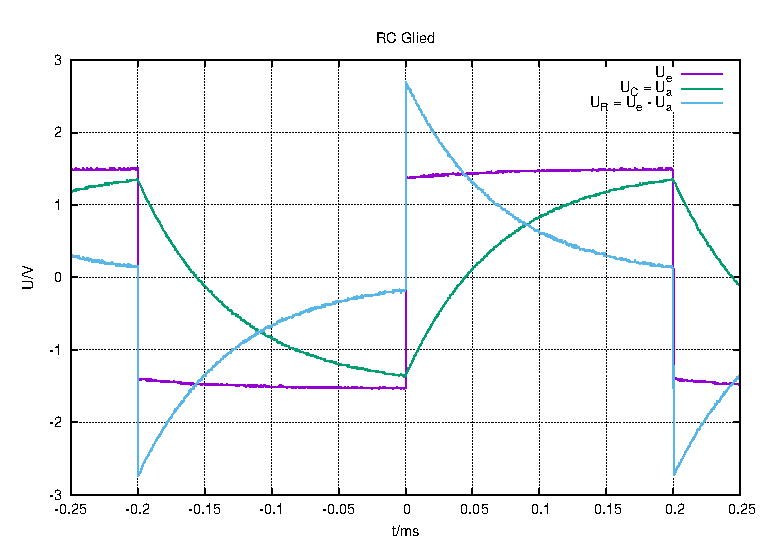
\includegraphics{graphics/CN_plot.eps}
    \caption{Spannungen im RC-Glied} \label{fig:RCplot}
\end{figure}

Das RC-Glied wird nach Schaltbild \ref{fig:RC} aufgebaut.
Die darin auftretenden Spannungen bei angelegter Rechteckspannung mit
$\nu=2.5~\mathrm{Hz}$, $R=1~\mathrm{\Omega}$ und $C=66~\mathrm{nF}$
sind in Abbildung \ref{fig:RCplot} aufgetragen.

Zur Messung der Zeitkonstante wird die anlegegte Pulsdauer vergrößert,
um vollständige Aufladung des Kondensators zu garantieren.
Die Messung von $U_{p-p}$ ergibt $U_{p-p}=3.025~\mathrm V$.
Folglich muss die Spannung am Kondensator innerhalb von $\tau$ auf
$e^{-1}\,U_{p-p}=1.113~\mathrm V$ abfallen.
Dies ist laut Messung bei folgendem Ergebnis der Fall:

\begin{equation*}
    \boxed{\tau\,=\,71~\mathrm{\mu s}}
\end{equation*}

\subsection {Kompensierter Spannungsteiler}

Der kompensierte Spannungsteiler wird nach Schaltbild \ref{fig:SPT} aufgebaut.
Zunächst wird der Stellwiderstand $R_2$ so eingestellt,
dass für das Verhältnis zwischen Ausgangs- und Eingangsspannung
$\frac{U_a}{U_e}=\frac{0.60~\mathrm{V}}{3.04~\mathrm{V}}\approx\frac{1}{5}$
gilt.
$U_e$ und $U_a$ sind für den kompensierten, über- und unterkompensierten Fall
in Abbildung \ref{fig:SPTplot} auf Seite \pageref{fig:SPTplot} aufgetragen.

\begin{figure}[!ht]
    \centering
    \begin{subfigure}{\textwidth}
        \centering
        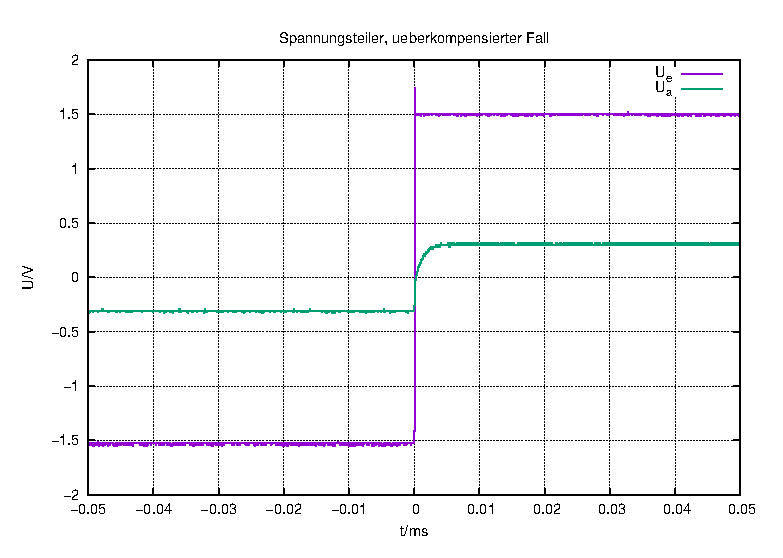
\includegraphics[width=0.7\textwidth]
            {graphics/spannungsteiler_ueberkomp.eps}
        \caption{überkompensierter Fall}
    \end{subfigure}
    \begin{subfigure}{\textwidth}
        \centering
        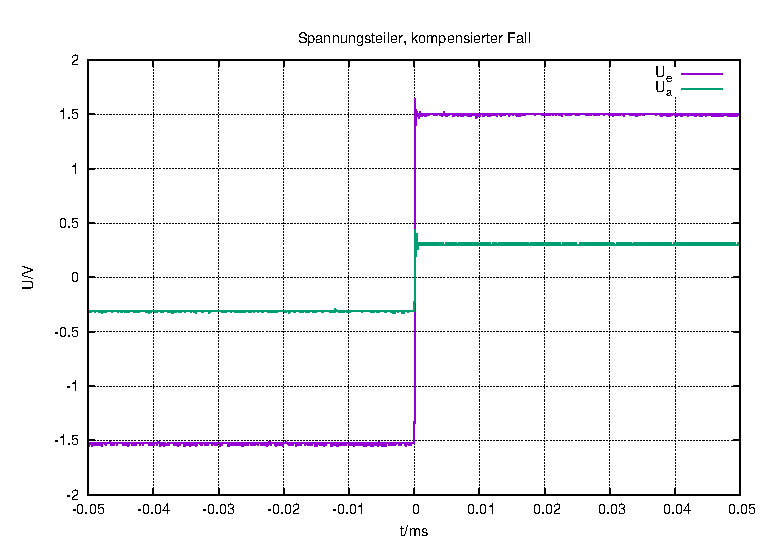
\includegraphics[width=0.7\textwidth]
            {graphics/spannungsteiler_komp.eps}
        \caption{kompensierter Fall}
    \end{subfigure}
    \begin{subfigure}{\textwidth}
        \centering
        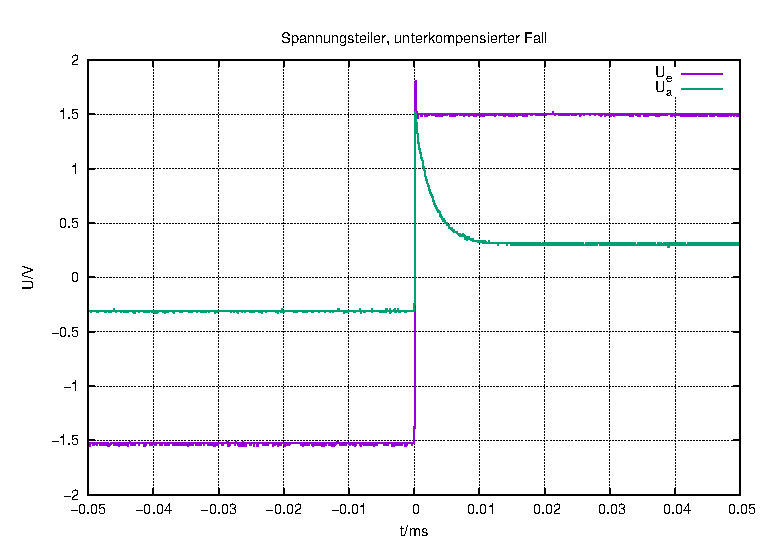
\includegraphics[width=0.7\textwidth]
            {graphics/spannungsteiler_unterkomp.eps}
        \caption{unterkompensierter Fall}
    \end{subfigure}
    \caption {zeitlichter Verlauf von $U_a$ und $U_e$ im Spannungsteiler}
    \label{fig:SPTplot}
\end{figure}

Zur weiteren Betrachtung der Verläufe wird nun auch noch eine
Fouriertransformation auf die Signale angewandt,
die in Abbildung \ref{fig:SPTplot_fourier} auf Seite
\pageref{fig:SPTplot_fourier} aufgetragen ist.

\begin{figure}[!ht]
    \centering
    \begin{subfigure}{\textwidth}
        \centering
        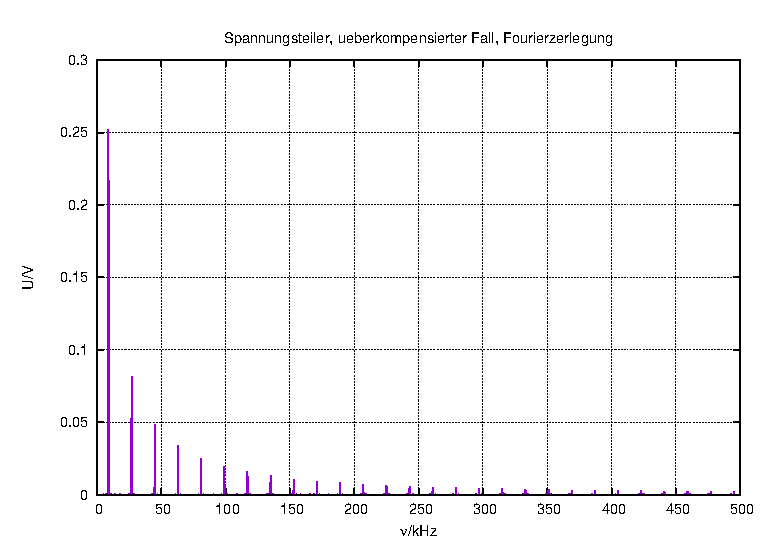
\includegraphics[width=0.7\textwidth]
            {graphics/spannungsteiler_ueberkomp_fourier.eps}
        \caption{überkompensierter Fall}
    \end{subfigure}
    \begin{subfigure}{\textwidth}
        \centering
        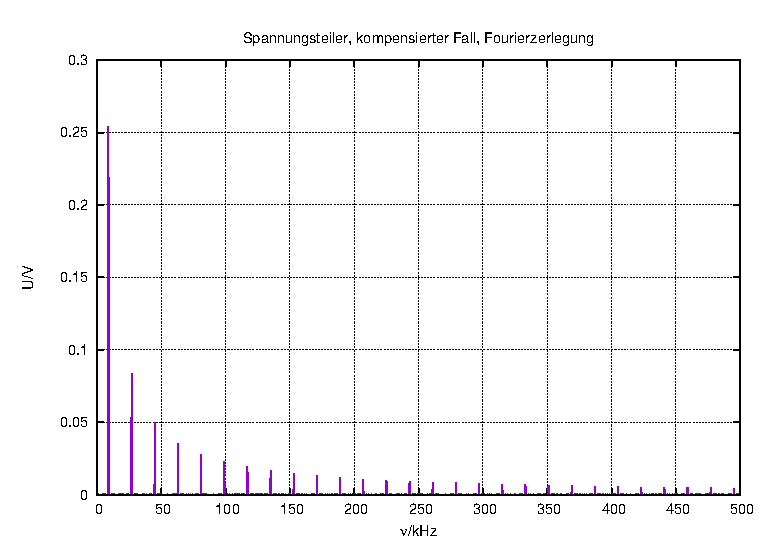
\includegraphics[width=0.7\textwidth]
            {graphics/spannungsteiler_komp_fourier.eps}
        \caption{kompensierter Fall}
    \end{subfigure}
    \begin{subfigure}{\textwidth}
        \centering
        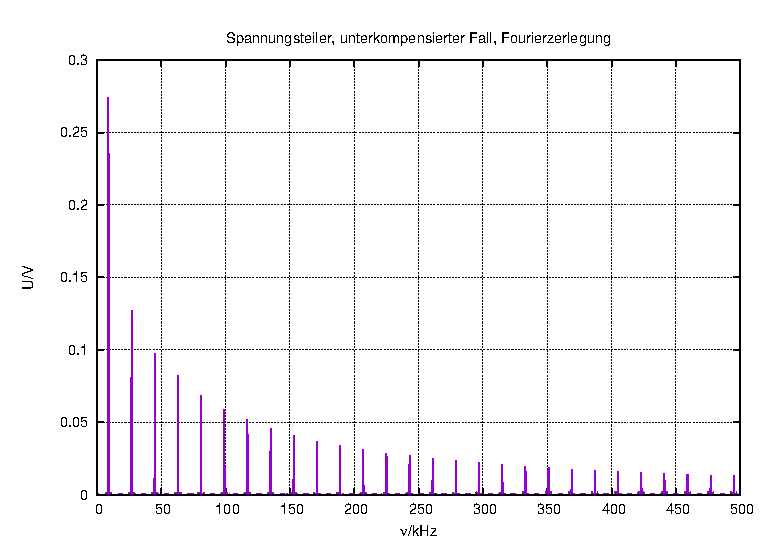
\includegraphics[width=0.7\textwidth]
            {graphics/spannungsteiler_unterkomp_fourier.eps}
        \caption{unterkompensierter Fall}
    \end{subfigure}
    \caption {Frequensspektrum von $U_a$ und $U_e$ im Spannungsteiler}
    \label{fig:SPTplot_fourier}
\end{figure}

\subsection {Tastkopf}

Der Tastkopf wird an das Oszilloskop angeschlossen und die Messspitze im
Comp Probe Ausgang des Oszilloskops angehangen.
Dort liegt $U_e$ als Rechteckspannung an.

Das Frequensspektrum des von $U_a$, das einer Fouriertransformation entspringt,
ist für kompensierten, über- und unterkompensierten Fall in
Abbildung \ref{fig:Tastkopf_fourier} auf Seite \pageref{fig:Tastkopf_fourier}
aufgetragen.

\begin{figure}[!ht]
    \centering
    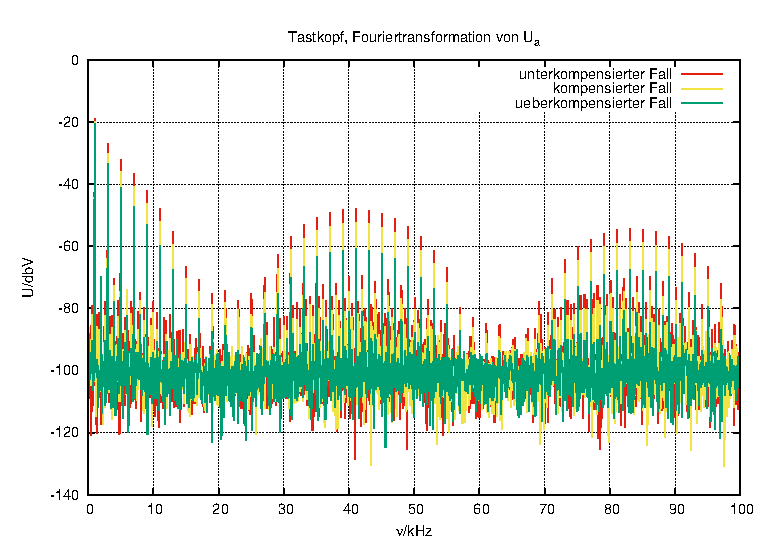
\includegraphics[width=\textwidth]{graphics/tastkopf.eps}
    \caption{Fouriertransformation von $U_a$ am Tastkopf}
    \label{fig:Tastkopf_fourier}
\end{figure}

\subsection {Wien-Brücke}

Am Oszilloskop werden die Frequenzen $\nu_i$ und Spannungen $U_{ei}$, $U_{ai}$
gleichzeitig für die Phasenverschiebungen $\phi_1=-\frac{\pi}{4}$, $\phi_2=0$
und $\phi_3=\frac{\pi}{4}$ gemessen.
Die Kondensatoren haben eine Kapazität von $C=10~\mathrm{nF}$ und die
Widerstände betragen $R=10~\mathrm{k\Omega}$.
Die Ergebnisse sind in Tabelle \ref{tb:Wien} protokolliert.

\begin{table}[!ht]
    \centering
    \caption{Phasenbeziehungen, Frequenzen und Spannungen am Wien-Brücken-Zweig}
    \label{tb:Wien}
    \begin{tabular}{c|r|r|r|r|r}
        $i$&$\phi_i/^\circ$&$\nu_i/\mathrm{kHz}$&$U_{ei}/\mathrm U$
        &$U_{ai}/\mathrm U$&$\left(\frac{U_a}{U_e}\right)_i$
        \\\hline
        1&$-45.6$&0.4899&3.02&0.72&0.24\\
        2&0.7&1.7094&3.00&0.99&0.33\\
        3&45.0&5.4980&3.00&0.70&0.23\\
    \end{tabular}
\end{table}

\section {Auswertung}

\subsection {RC-Glied}

Die Betrachtung des RC-Gliedes lieferte die folgenden Ergebnisse:

\begin{empheq}[box=\fbox]{align}
    \tau_{th}\,&=\,66.7~\mathrm{\mu s}\\
    \tau\,&=\,71~\mathrm{\mu s}
\end{empheq}

Theoretisches Ergebnis $\tau_{th}$ und gemessenes Ergebnis $\tau$ liegen hierbei
in einer Größenordnung und unterscheiden sich lediglich um etwa
$4~\mathrm{\mu s}$.
Gemessen an $\tau$ ist dies eine Abweichung von $5.7\%$ und liegt in einem
Bereich, bei dem man noch sagen kann, dass die gemessenen Ergebnisse den
erwarteten entsprechen.

Die leichte Erhöhung von $\tau$ gegenüber dem theoretischen Wert kommt
vermutlich durch zusätzliche Kapazitäten und Widerstände in Kabeln
und Messgeräten zustande.
Auch wenn diese gering sind, kann der Einfluss in der Formel $\tau=RC$
ein größerer sein.

\subsection {Kompensierter Spannungsteiler}

Deutlich sichtbar ist, dass im kompensierten Fall das ausgehende Signal mit dem
eingehenden bis auf die Amplitude ziemlich übereinstimmt,
es ist wieder eine Rechteckspannung.
Im überkompensierten Fall jedoch ist der Vorzeichenwechsel stark abgedämpft,
was in einem abgerundeten Übergang resultiert.
Im unterkompensierten Fall hingegen ist das Gegenteil sichtbar,
das Signal schwingt beim Vorzeichenwechsel über und resultiert in einem
spitzen Peak.

Dies ist auch in der Fourieranalyse gut sichtbar.
Während der Unterkompensierte Fall viele Frequenzen notwendig sind,
um den Peak im Signal zu bilden, genügen beim Rechteckpuls bereits weniger
Frequenzen, die Peaks im Frequensspektrum sind also geringer.
Im überkompensierten Fall hat man einen abgerundeten Übergang,
für den erneut weniger Frequenzen notwendig sind.
Auch dies zeigt sich durch die Fouriertransformation.

Dies macht die eingangs erwähnten Effekte des Spannungsteilers deutlich.
Die Spannung vom Eingangssignal ist stärker als die des Ausgangssignales,
was einem erhöhten Widerstand am Messgerät analog ist.
Die korrekt gewählte Kapazität sorgt dafür,
dass das Signal bei Schaltsprüngen nicht überschwingt (unterkompensiert) und
auch nicht erst zum Endwert hinkriecht (überkompensiert).

\subsection {Tastkopf}

Das gleiche Verhalten ist auch am Tastkopf zu sehen,
der mit dem Oszilloskop ebenfalls einen Spannungsteilers bildet.
Im überkompensierten Fall sind die Werte für größere Frequenzen deutlich
geringer als im kompensierten Fall und im unterkompensierten sind sie am
für größere Frequenzen am größten.

\subsection {Wien-Brücke}

Das erwartete Verhältnis von $\left(\frac{U_a}{U_e}\right)_{th}=\frac{1}{3}$
entspricht dem gefundenen $\left(\frac{U_a}{U_e}\right)_2=0.33$ für die
Phasenverschiebungen $\phi_2=0.7^\circ\approx0$.
Diese Phasenverschiebungen liegt bei $\nu_2=1.7~\mathrm{kHz}$.
Der theoretische Wert dieser Frequenz beträgt
$\nu_{th}=\frac{1}{2\pi\,RC}=1.6~\mathrm{kHz}$.
Theoretischer und praktisch ermittelter Wert liegen dicht beieinander.

Auch zu beobachten ist, dass die Werte $U_{a1}$ und $U_{a3}$ für die
Phasenrelationen $\phi_{1,2}\approx\pm45^\circ$ nah beieinander liegen,
was eine Symmetrie der Spannung bezüglich der Phasenrelation vermuten lässt.
Beide Spannungen liegen unterhalb von $U_{a2}$ für $\phi_2\approx0$,
was daran liegt, dass es sich um einen Bandpass handelt,
der von $\nu_2$ verschiedene Frequenzen abschwächt.

% \pagebreak
% \section {Quellen}
% \begin{thebibliography}{999}
% \bibitem {WalterHerms} G. Walter und G. Herms, Einführung in die Behandlung von Messfehlern -- Ein Leitfaden für das Praktikum der Physik, Universität Rostock 2006d
% \end{thebibliography}

\section {Anhang}

\begin{table}[ht!]
    \centering
    \caption{verwendete Geräte} \label{tab:devices}
    \begin{tabular}{lr}
        Arbeitsplatz & 9\\
        RC-Modul&10\\
        Oszilloskop&Agilent Technologies Infiicision MSO-X 2002A\\
        Mini $\Omega$ Dekade&RT 1-1000 SAB\\
        Mini C Dekade&Cosinus C1-250 SAB\\
        Tastkopf&Agilent N2862B Passive Probe
    \end{tabular}
\end{table}


\end{document}
%sagemathcloud={"zoom_width":100}
